\begin{figure}[!htb]
    % \centering
    \Subfigure[0.49]{\includegraphics[width=1\textwidth]{figures/simulations/collisional/CD+_He_f-time__transition_0-1_0.001s_population_ratio.pdf}}{}{\label{fig:ROSAA-sim-collisional}}
    \hfill
    \Subfigure[0.49]{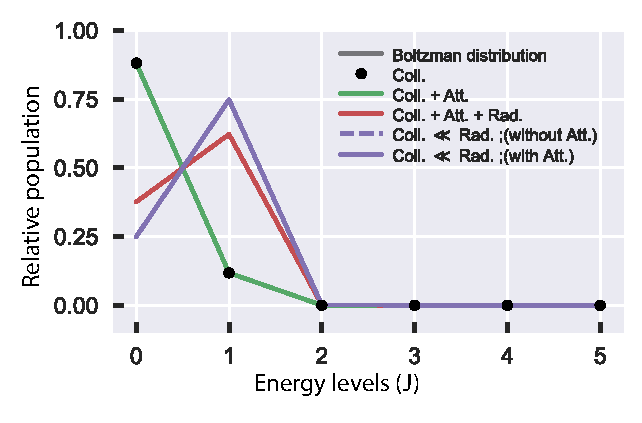
\includegraphics[width=1\textwidth]{figures/simulations/collisional/CD+_He_f-time__transition_0-1_0.001s_boltzman_comparision.pdf}}{}{\label{fig:ROSAA-sim-collisional-boltzmann}}
    
    \caption{(a) Collisional process for \CD ions up to $J=5$ with He buffer gas ([He]$=2.2 \cdot 10^{14}$ \percc). The coloured label indicates the corresponding \CD$(J)$ state. At $t=0$, T$_{coll}=300$ K, at which the relative population corresponds to a Boltzmann distribution at 300 K. The relative population evolves through collisions with He with rate constants for T$_{coll}=7$ K (derived from \cite{Werfelli2017}), subsequently reaching equilibrium after $<0.5$ ms. (b) Comparison of the Boltzmann distribution at 7 K with the relative population involving only collisional process (Coll.) at $t=1$ ms.}
    \label{fig:ROSAA-sim-collisional-boltzman-comparision}
\end{figure}